\chapter{System Design}
The following chapter will briefly explain the chosen design process for the project. The components of the project are broken into four parts: Data Preparation for insight into the data utilized and how it will be prepared, A section on what algorithm and machine learning library will be used, an explanation on the approach for training the model and a Deployment section for the process in which the model was deployed for production. Lastly, the overall system architecture and flow of objectives will be explained.

\section{Data Preparation}
As stated by \citeauthor*{LOPES} that there is a scarcity of public datasets with for facial expression images, therefore the Cohn-Kanade+ (CK+) dataset shall be used as it provides a wide range of emotions to train the model on. However, in the emotion of disgust and contempt will be omitted from the project as it does not fit the nature of the use case, and they bear too much resemblance to the anger images. Instead, a neutral emotion class will be implemented.
The dataset will be preprocessed to reduce dimensionality, and synthetic samples will be generated via data augmentation to increase the size of the dataset and prevent class imbalance. The dataset will then be divided into training and testing sets using split validation. 

\section{Machine Learning Model}
For designing the model, the Tensorflow Machine Learning library by Google will be used to design a convolutional neural network. 
The network consists of several convolution layers, three max pooling layers and a fully-connected layer. The model has six outputs nodes that provide classification for each emotion in the dataset. The model uses supervised learning, with labels for the images it was training on, which will be brought forward in the following section.\\

\section{Training}
Due to insufficient hardware, the approach of cloud training is needed in order to train the model. The Python code and the dataset are pushed to a containerized TensorFlow environment on the FloydHub cloud platform. The output of the trained model is saved to a Tensorflow \textit{.ckpt} file.

\section{Deployment}
In order to deploy the trained model to production, a Python API was developed using the Flask package, which is a library for running python code on a server. The API is hosted on Heroku PaaS as they provide an easy-to-use and free basic tier service for hosting Python applications. The trained model files are also deployed with the API. These model is read and initialized from the respective files when the API successfully build and deploys. The API accepts 'POST' requests and takes the image as input. The image is then fed into the model and a classification is made, this is then returned to the original sender.

Secondly, a Node.JS web app was developed in order to display how this model can be used in production. The application was also deployed to Heroku. The application uses the clients web cam in order to record their face. This takes snapshots of the users face and sends the images to the Python API in one second intervals. The application then receives the response from the API and displays it to the screen. 
See Figure \ref{ui} for a general design of the user interface for the node application.


\begin{figure}[ht]
	\begin{center}
		\advance\leftskip-3cm
		\advance\rightskip-3cm
		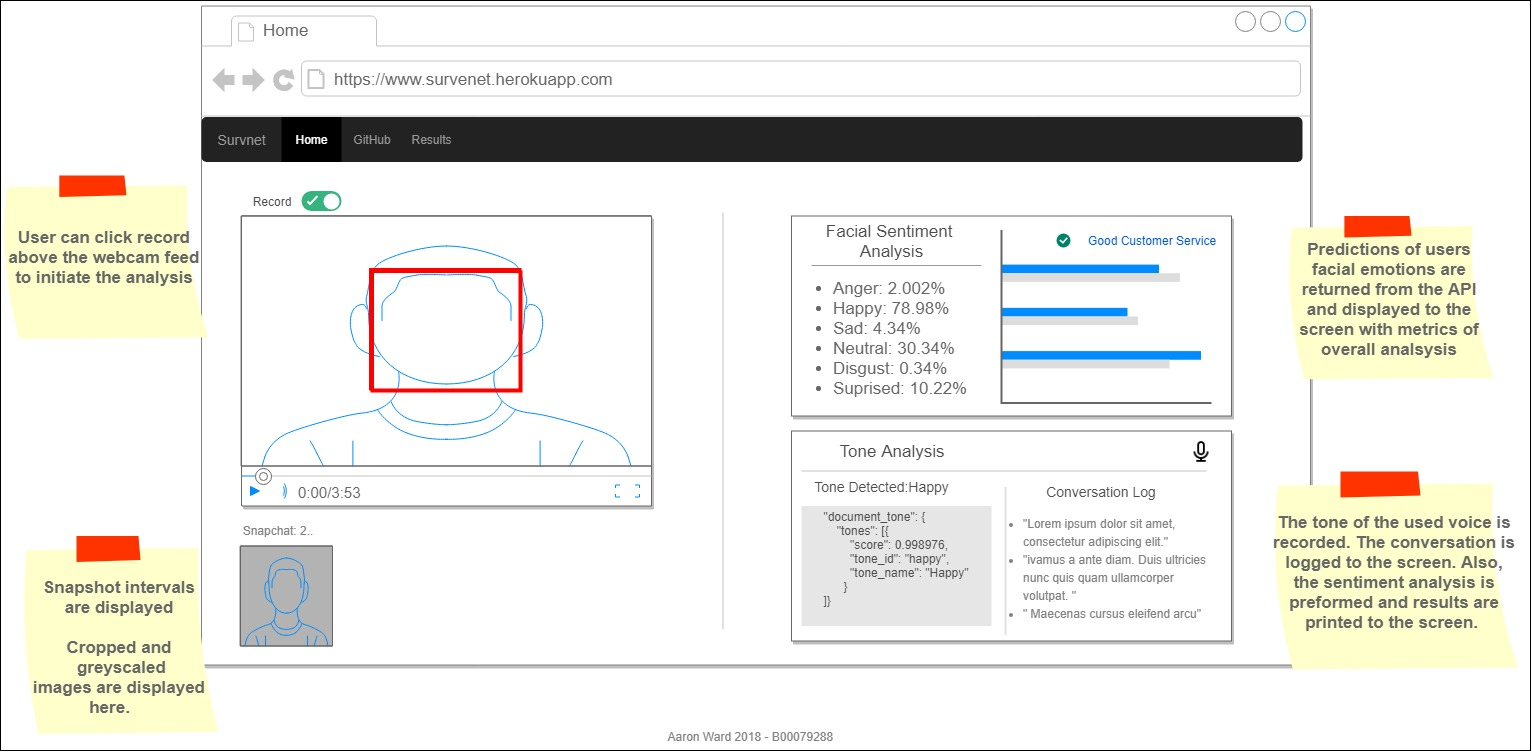
\includegraphics[keepaspectratio=true,scale=0.35]{__resources/Design/mockup_annotated.jpg}
		\caption{User Interface Design For Web Application}
		\label{ui}
	\end{center}
\end{figure}


\section{Concluding Remarks of System Architecture Design}
In summary, the system architecture will be considered in two parts: Training and deployment. Firstly, the data preparation and neural network scripts shall be written on a local machine. These scripts and dataset will be uploaded to a Tensorflow environment for training on the Flyodhub cloud service. Upon completion of training, the model will be saved and pushed to the \textit{model-serve} GitHub repository that is integrated with the Heroku PaaS. This repository consists of a Python Flask API to accept POST requests. The Node.js web application shall also be deployed to the Heroku for easy user access. This shall send requests to the model API for classification of images of the user.
Please refer to Figure \ref{arch} to see an illustrated tolopogy of the system.

\begin{figure}[ht]
	\begin{center}
		\advance\leftskip-3cm
		\advance\rightskip-3cm
		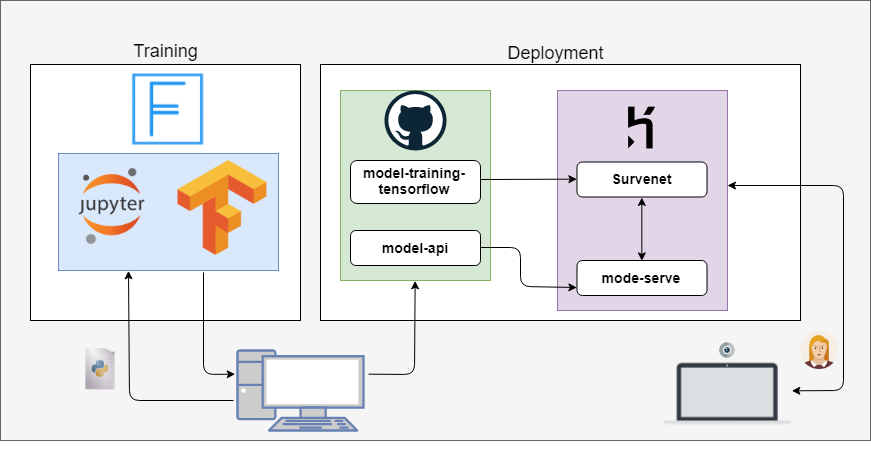
\includegraphics[keepaspectratio=true,scale=0.55]{__resources/Design/arch.png}
		\caption{System Architecture of Training and Deployment}
		\label{arch}
	\end{center}
\end{figure}

